\documentclass[../main.tex]{subfiles}
 
\begin{document}

\section{Saturday}

On Saturday you wake up happy that you managed to snatch 8 hours of sleep before your first day. You tend to experience sleep anxiety, so you hope to keep this up throughout the week. You pack your slim messenger bag and are soon walking out the front door to the Uber driver stopped in the middle of the street. There was literally one car available at 7:30am near your neighborhood. Leaving the cul-de-sac, you hope your 6 mile Uber commute won't become a problem throughout the week, as you now rely on the service. The dollars spent on the commute are nothing compared to the cost of a nice hotel within walking distance of the convention center. You tip well to maintain your rating, and because you should tip.

\begin{figure}[h]
	\centering
	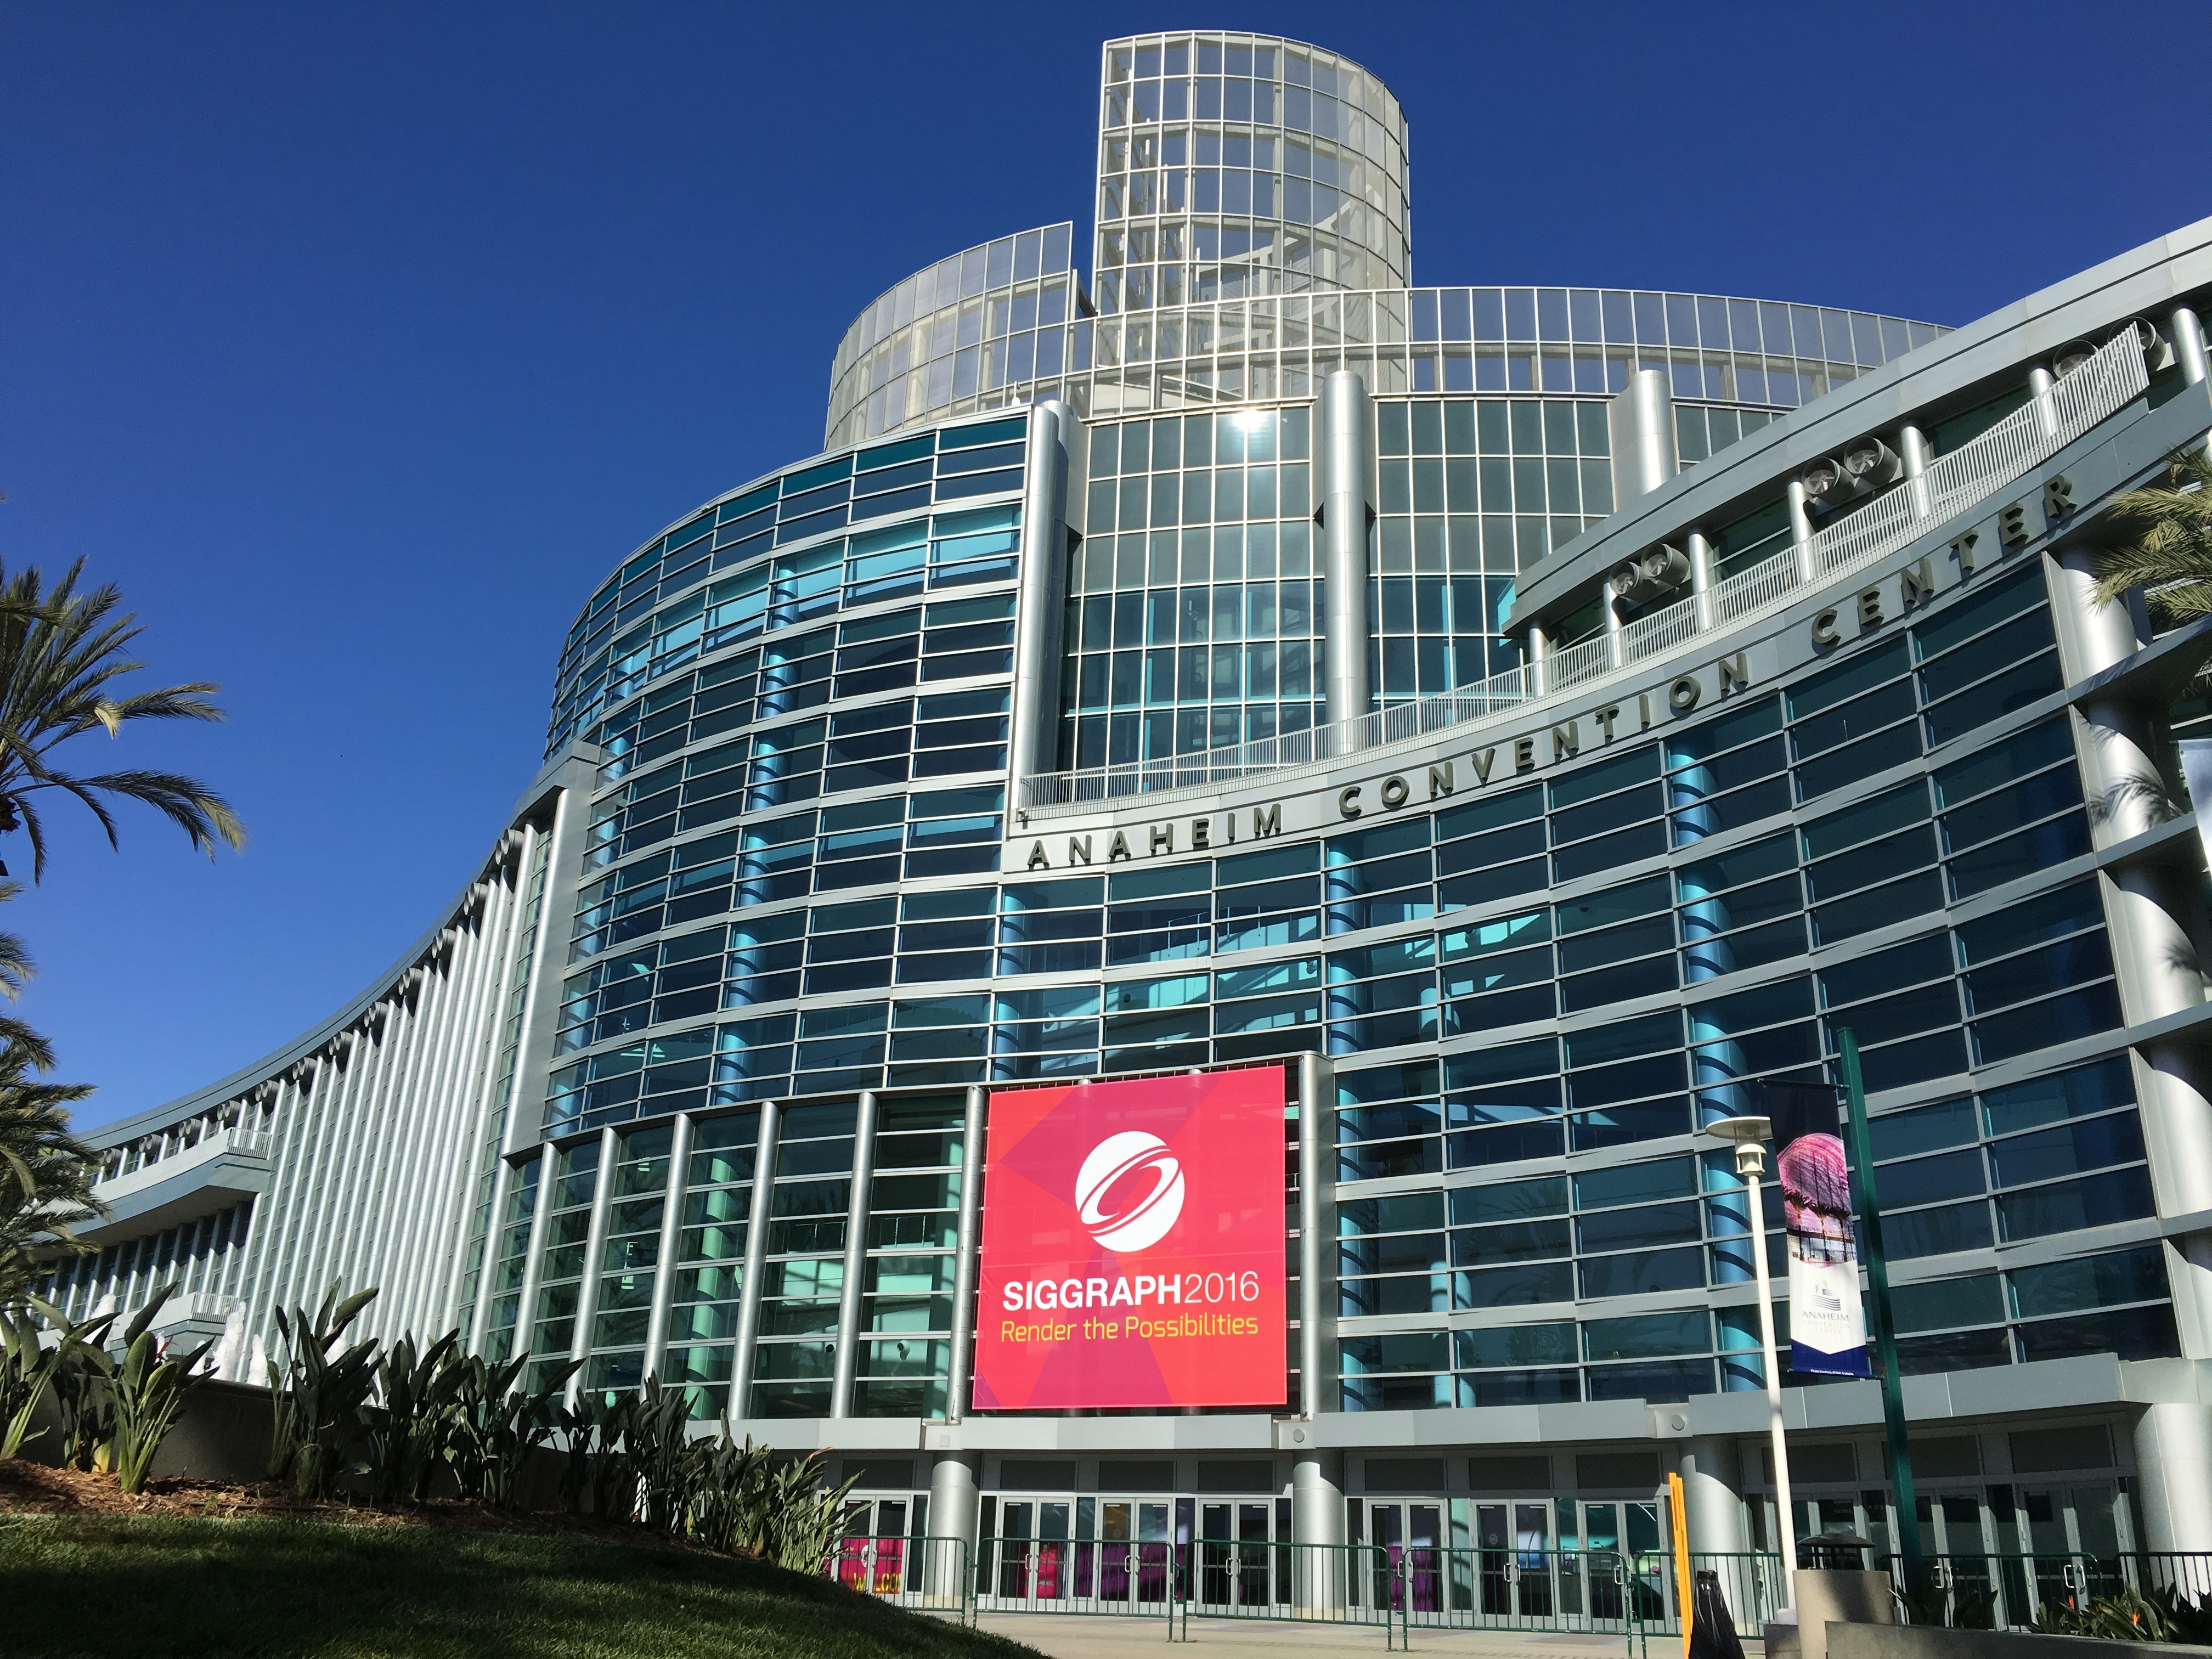
\includegraphics[width=\textwidth]{convention_center}
	\caption*{The Anaheim Convention Center.}
\end{figure}

You snacked instead of eating a proper dinner the previous night. After overdoing it with breakfast at Park 55 just down the street from the Anaheim Convention center, you make your way to the second floor's makeshift Student Volunteer office, where you plop yourself down on one of the many bean bag chairs in the back of the large room and continue working through \textit{Pit Bull} to pass the few hours that remain before noon check-in. You are not quite sure what security will be involved throughout the week and are a bit surprised that you could just walk into the building and into the SV office. Actually, from what you recall of your online training, many SVs will be end up \textit{being} the security. You are quite early. Other SVs will be getting off the plane and booking it to the convention center for check-in, which is mandatory and if missed may result in forfeiture of your badge. But you are way early. You hold off on diving into introductions with the few other SVs lounging about, keeping to yourself.

\begin{figure}[h]
	\centering
	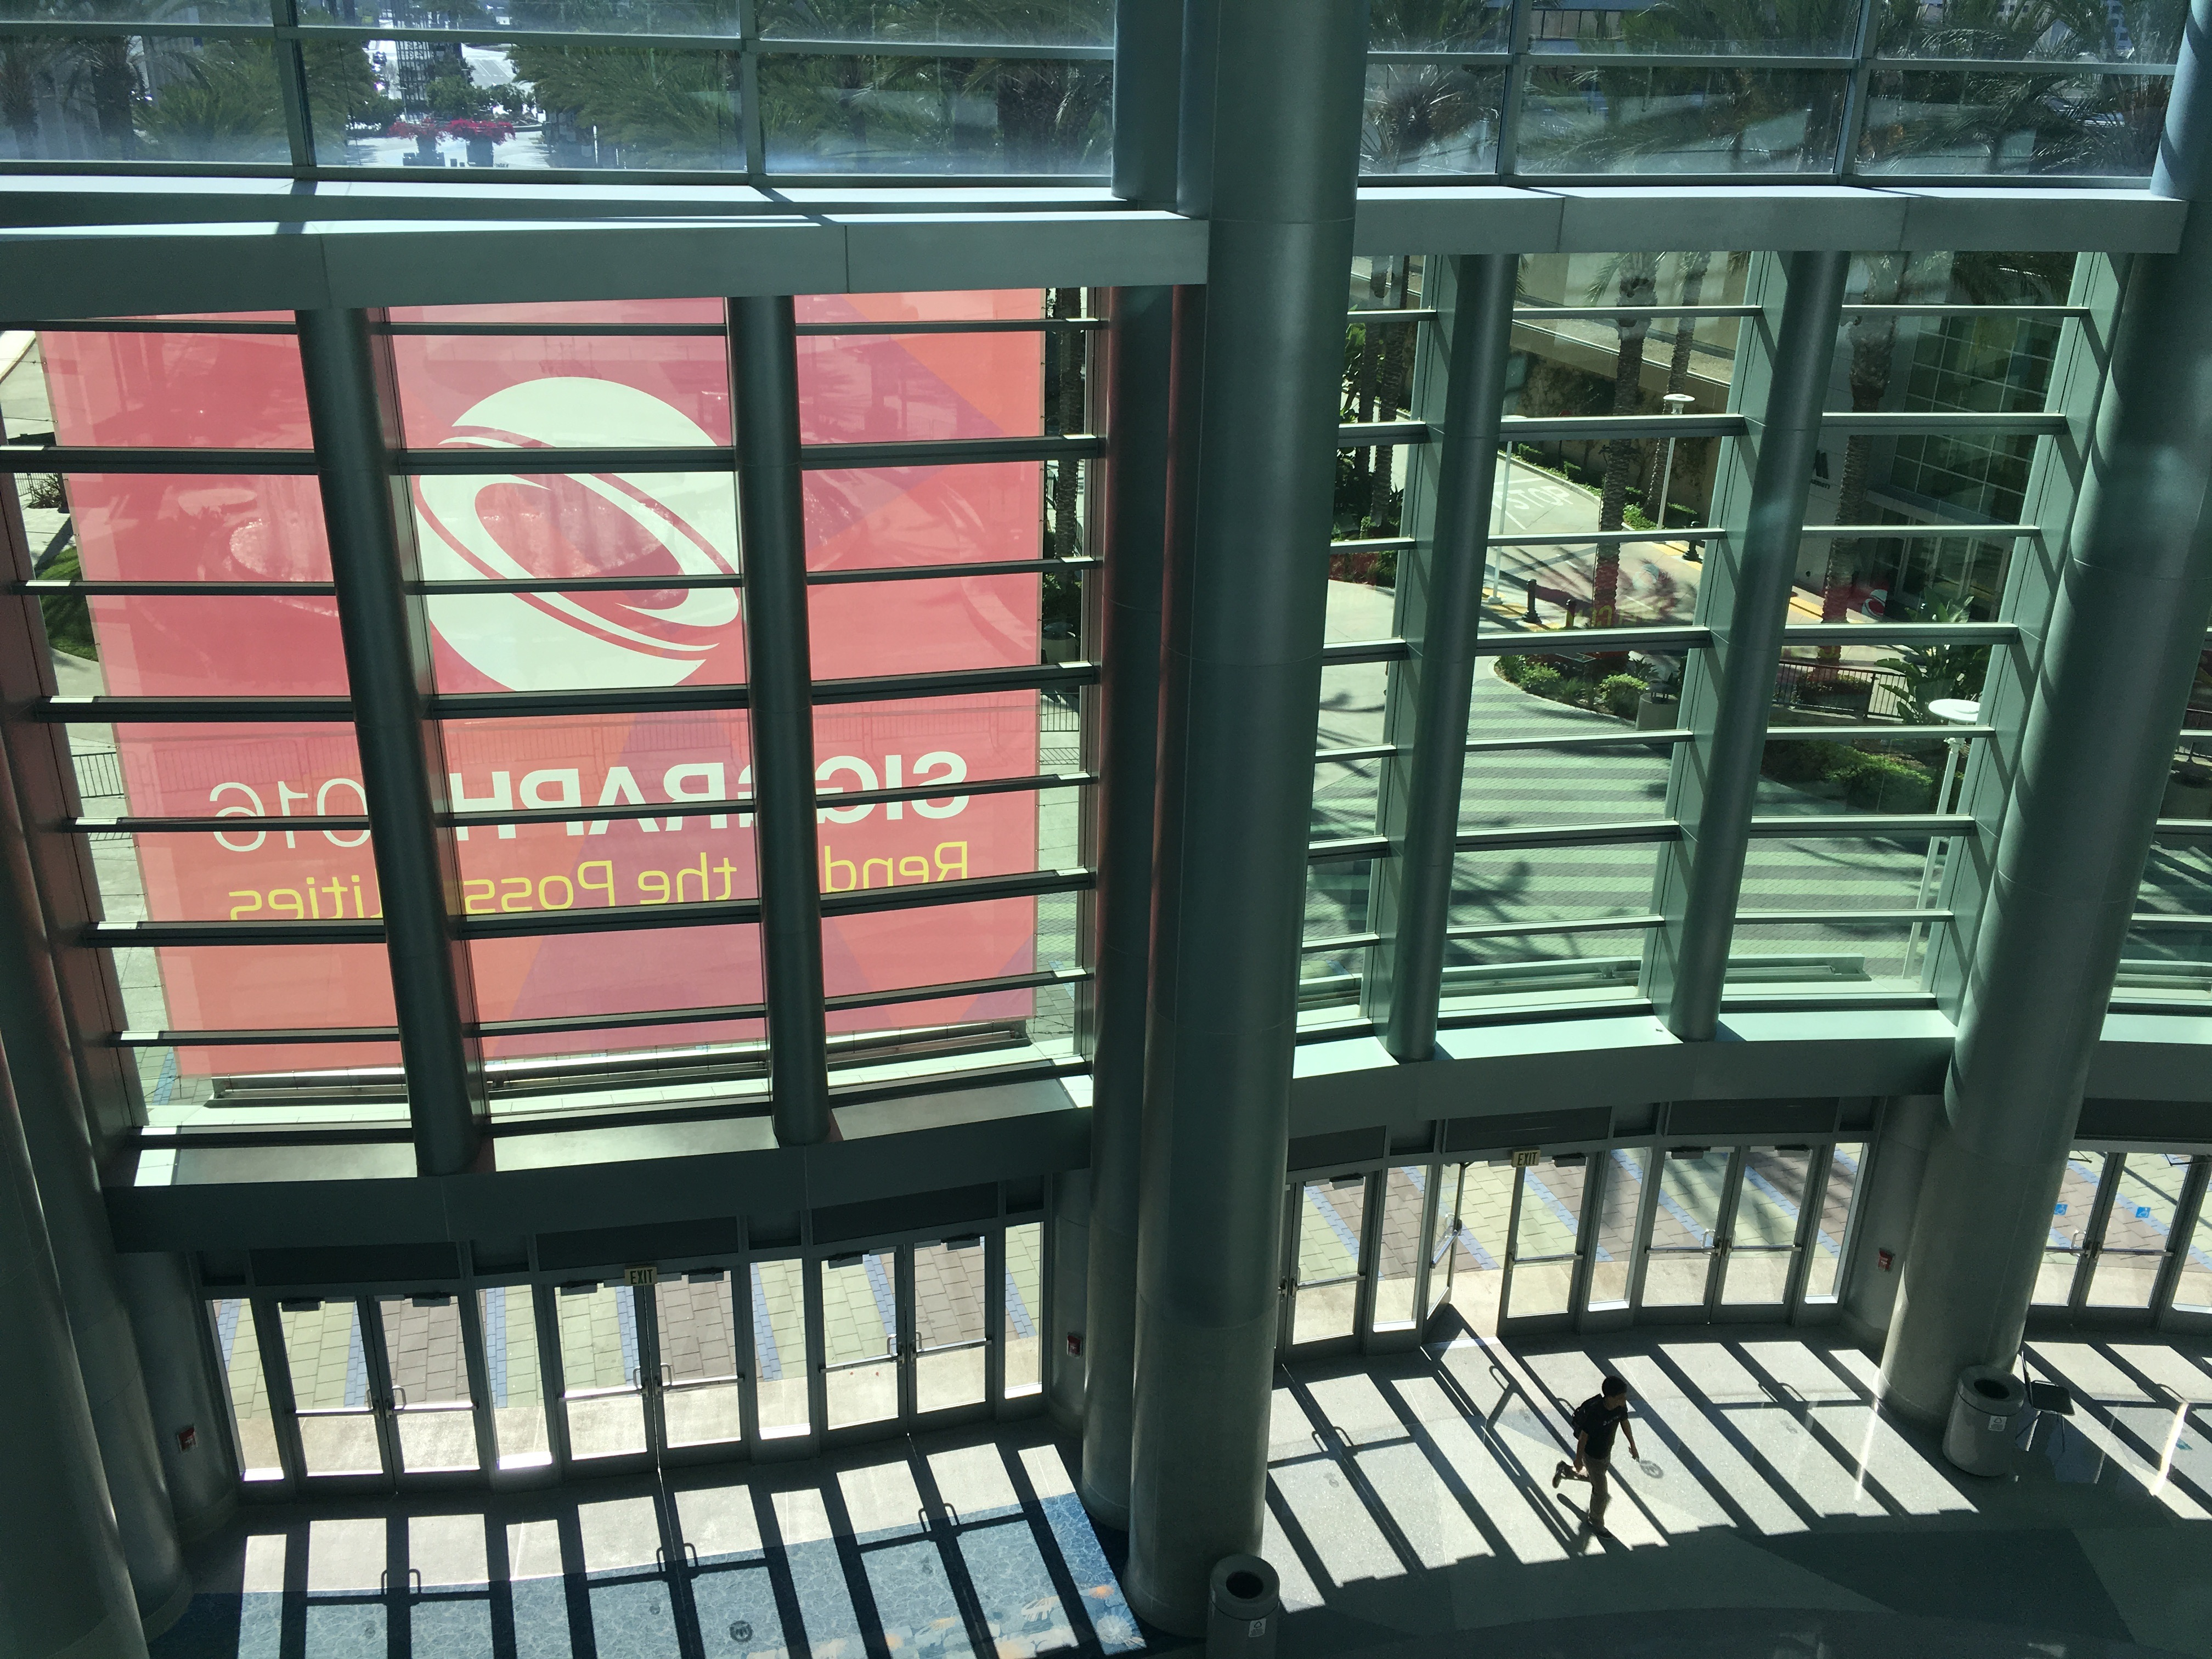
\includegraphics[width=\textwidth]{convention_center_inside}
	\caption*{A view from inside the Convention Center. Second Floor walkway.}
\end{figure}

Before long, you are recruited to help out on the main showroom, guided by a \textit{Team Leader} wearing a purple Dreamworks shirt (sporting the newly designed logo) and holding a clipboard and a walkie talkie. You worry about missing your prime spot in the registration line, but you know the name of the game here is to say yes, so you gather your bag and assemble with a handful of other early birds to lend a hand downstairs. For the next two hours, you load a couple thousand packets of papers and other goodies into tote bags that will be handed out to attendees. Each has on one side \textit{SIGGRAPH 2016} and this year's slogan: \textit{Render the Possibilities} over the tesselations and network symbology used for this year's promotional graphics. \textit{NJIT} is printed on the other side.

\begin{figure}[h]
	\centering
	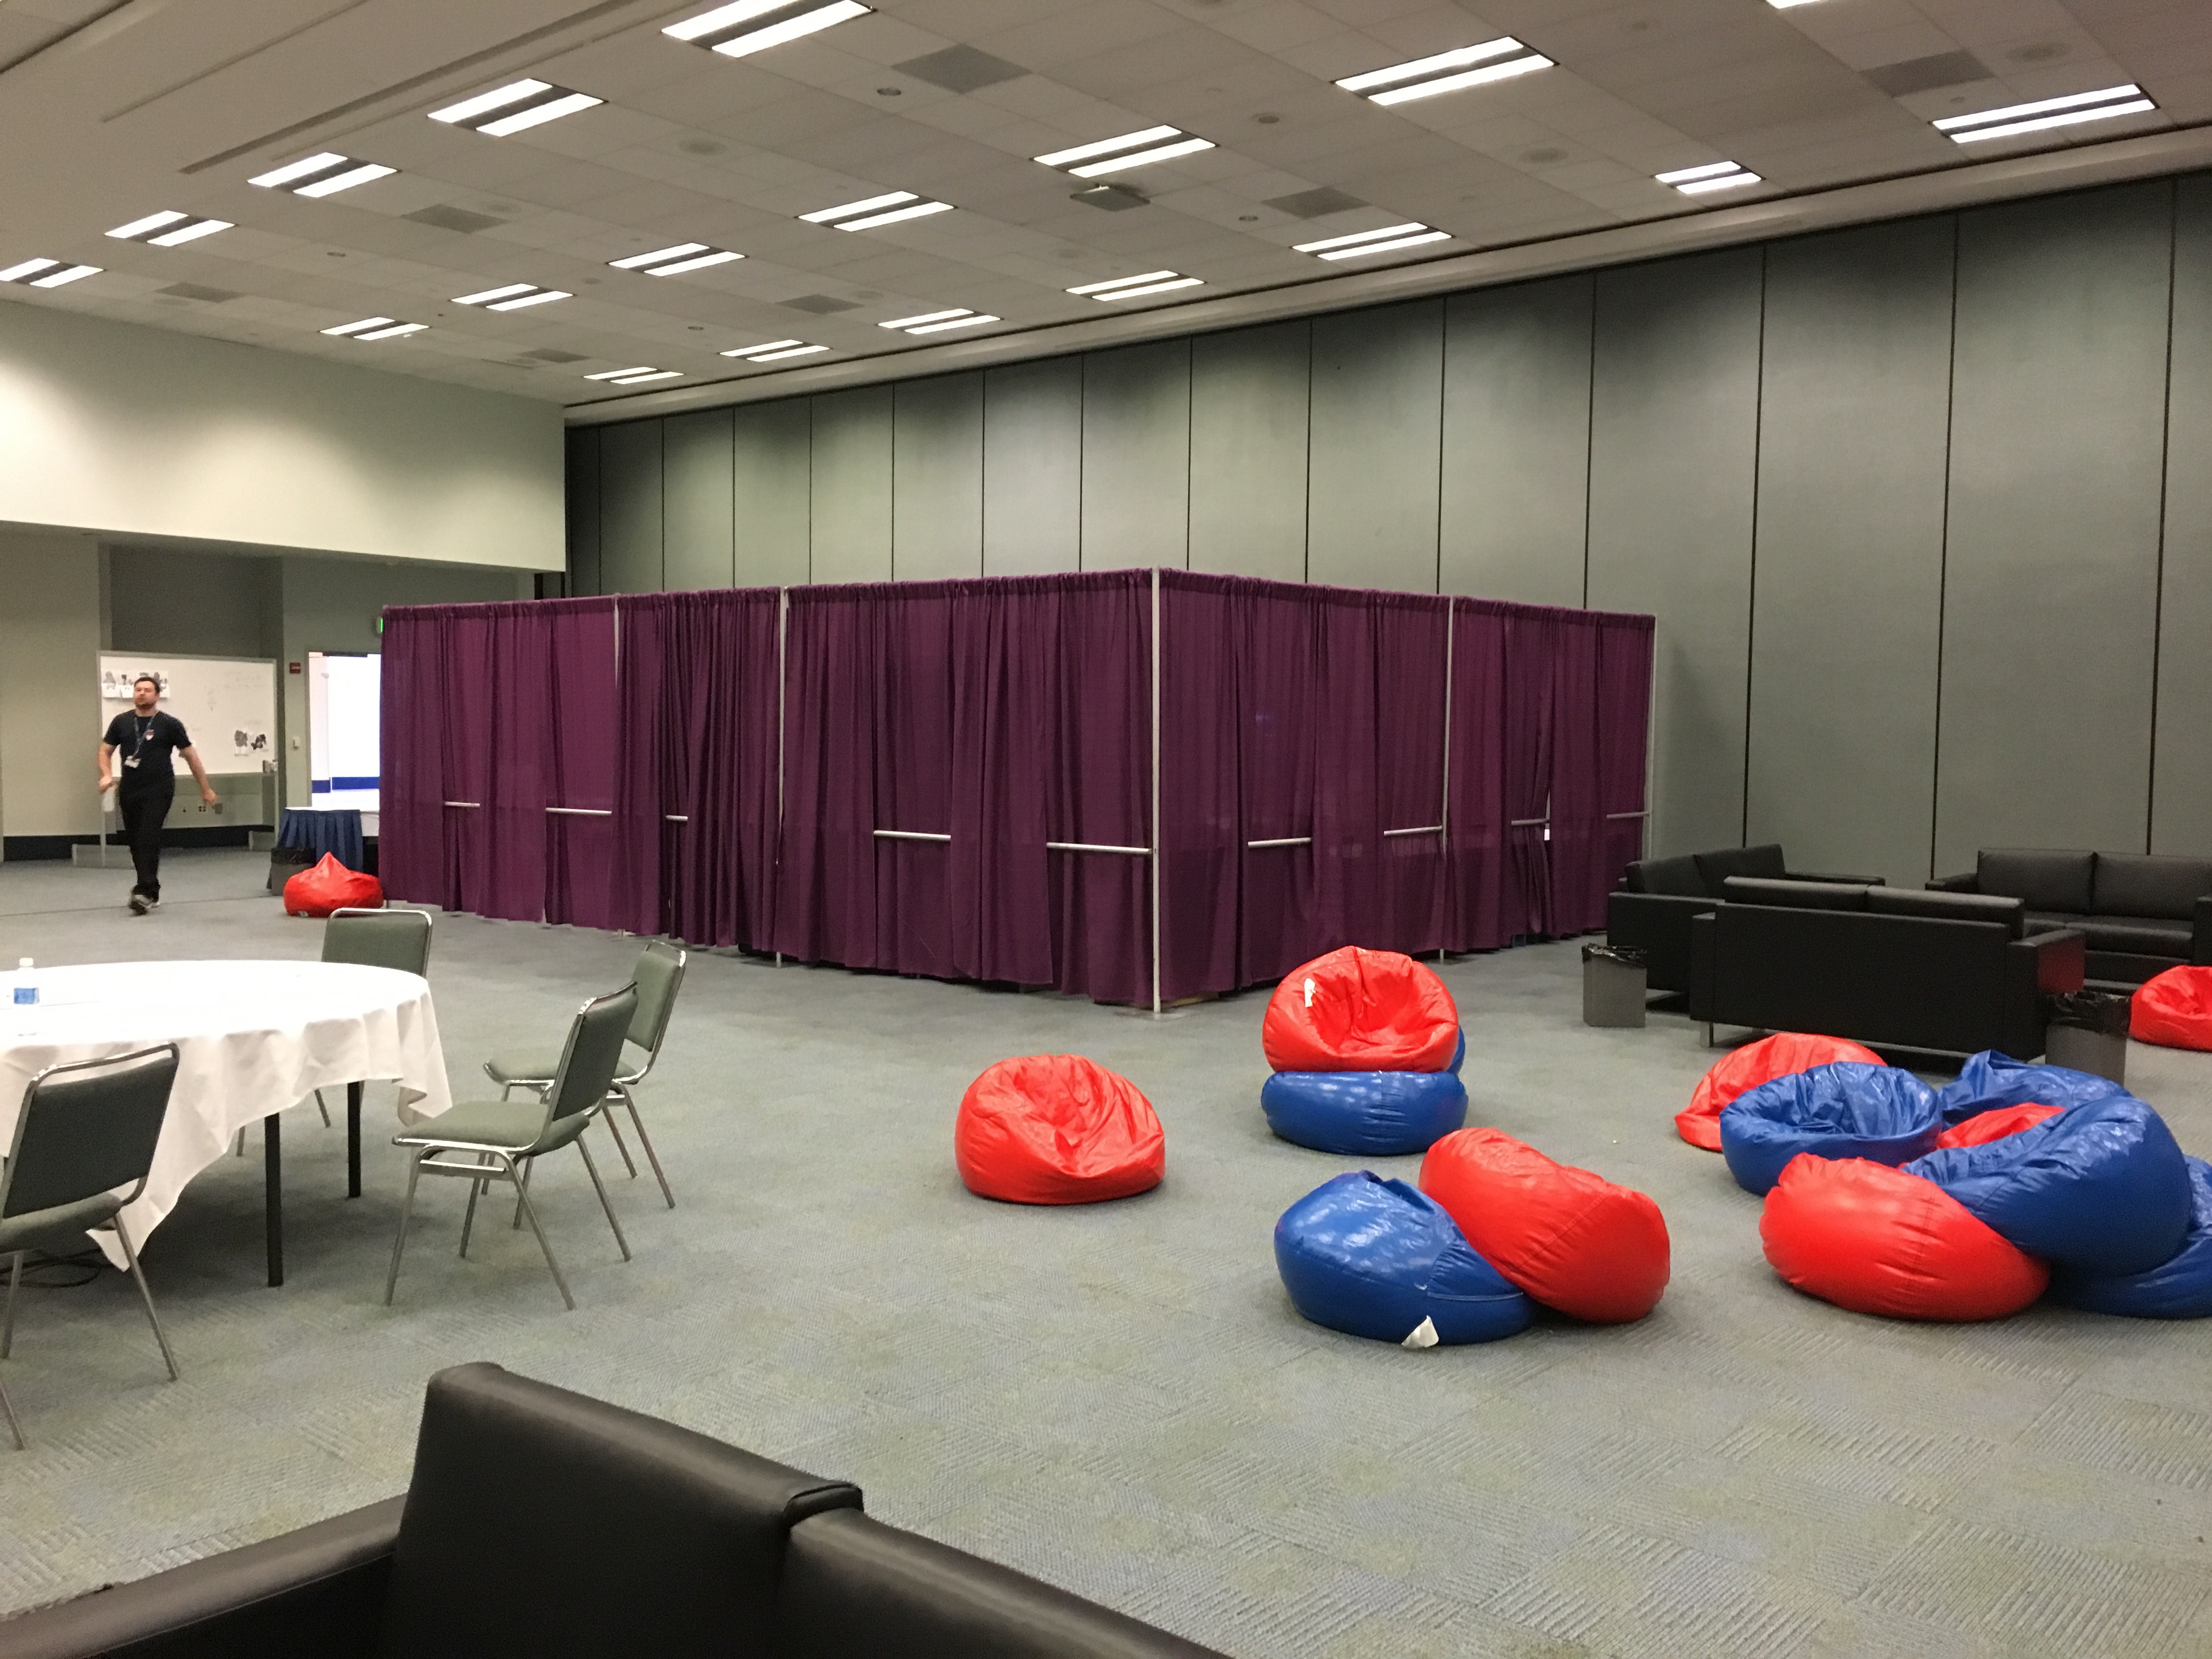
\includegraphics[width=\textwidth]{sv_office}
	\caption*{Student Volunteer Office.}
\end{figure}

This tote-bag-assembly line forms in Exhibition Hall, where companies will tout their products as well as recruit technical and artistic talent later in the week. It also houses registration tables, a merchandise corner for all things SIGGRAPH related, and an area where tickets for exclusive events may be swapped throughout the week. Cardboard boxes containing merchandise and miscellaneous equipement abound. The job fair is not set to open until Tuesday, you are told, and security guards dressed as valets stand around to make sure you don't wander too far back into the staging areas where companies are setting up booths. You saw Maxon, Nividia, and Intel banners when you first walked into the huge showroom floor. You begin feeling the excitement that must come at the very beginning of big conferences, before the weariness sets in.

\begin{figure}[h]
	\centering
	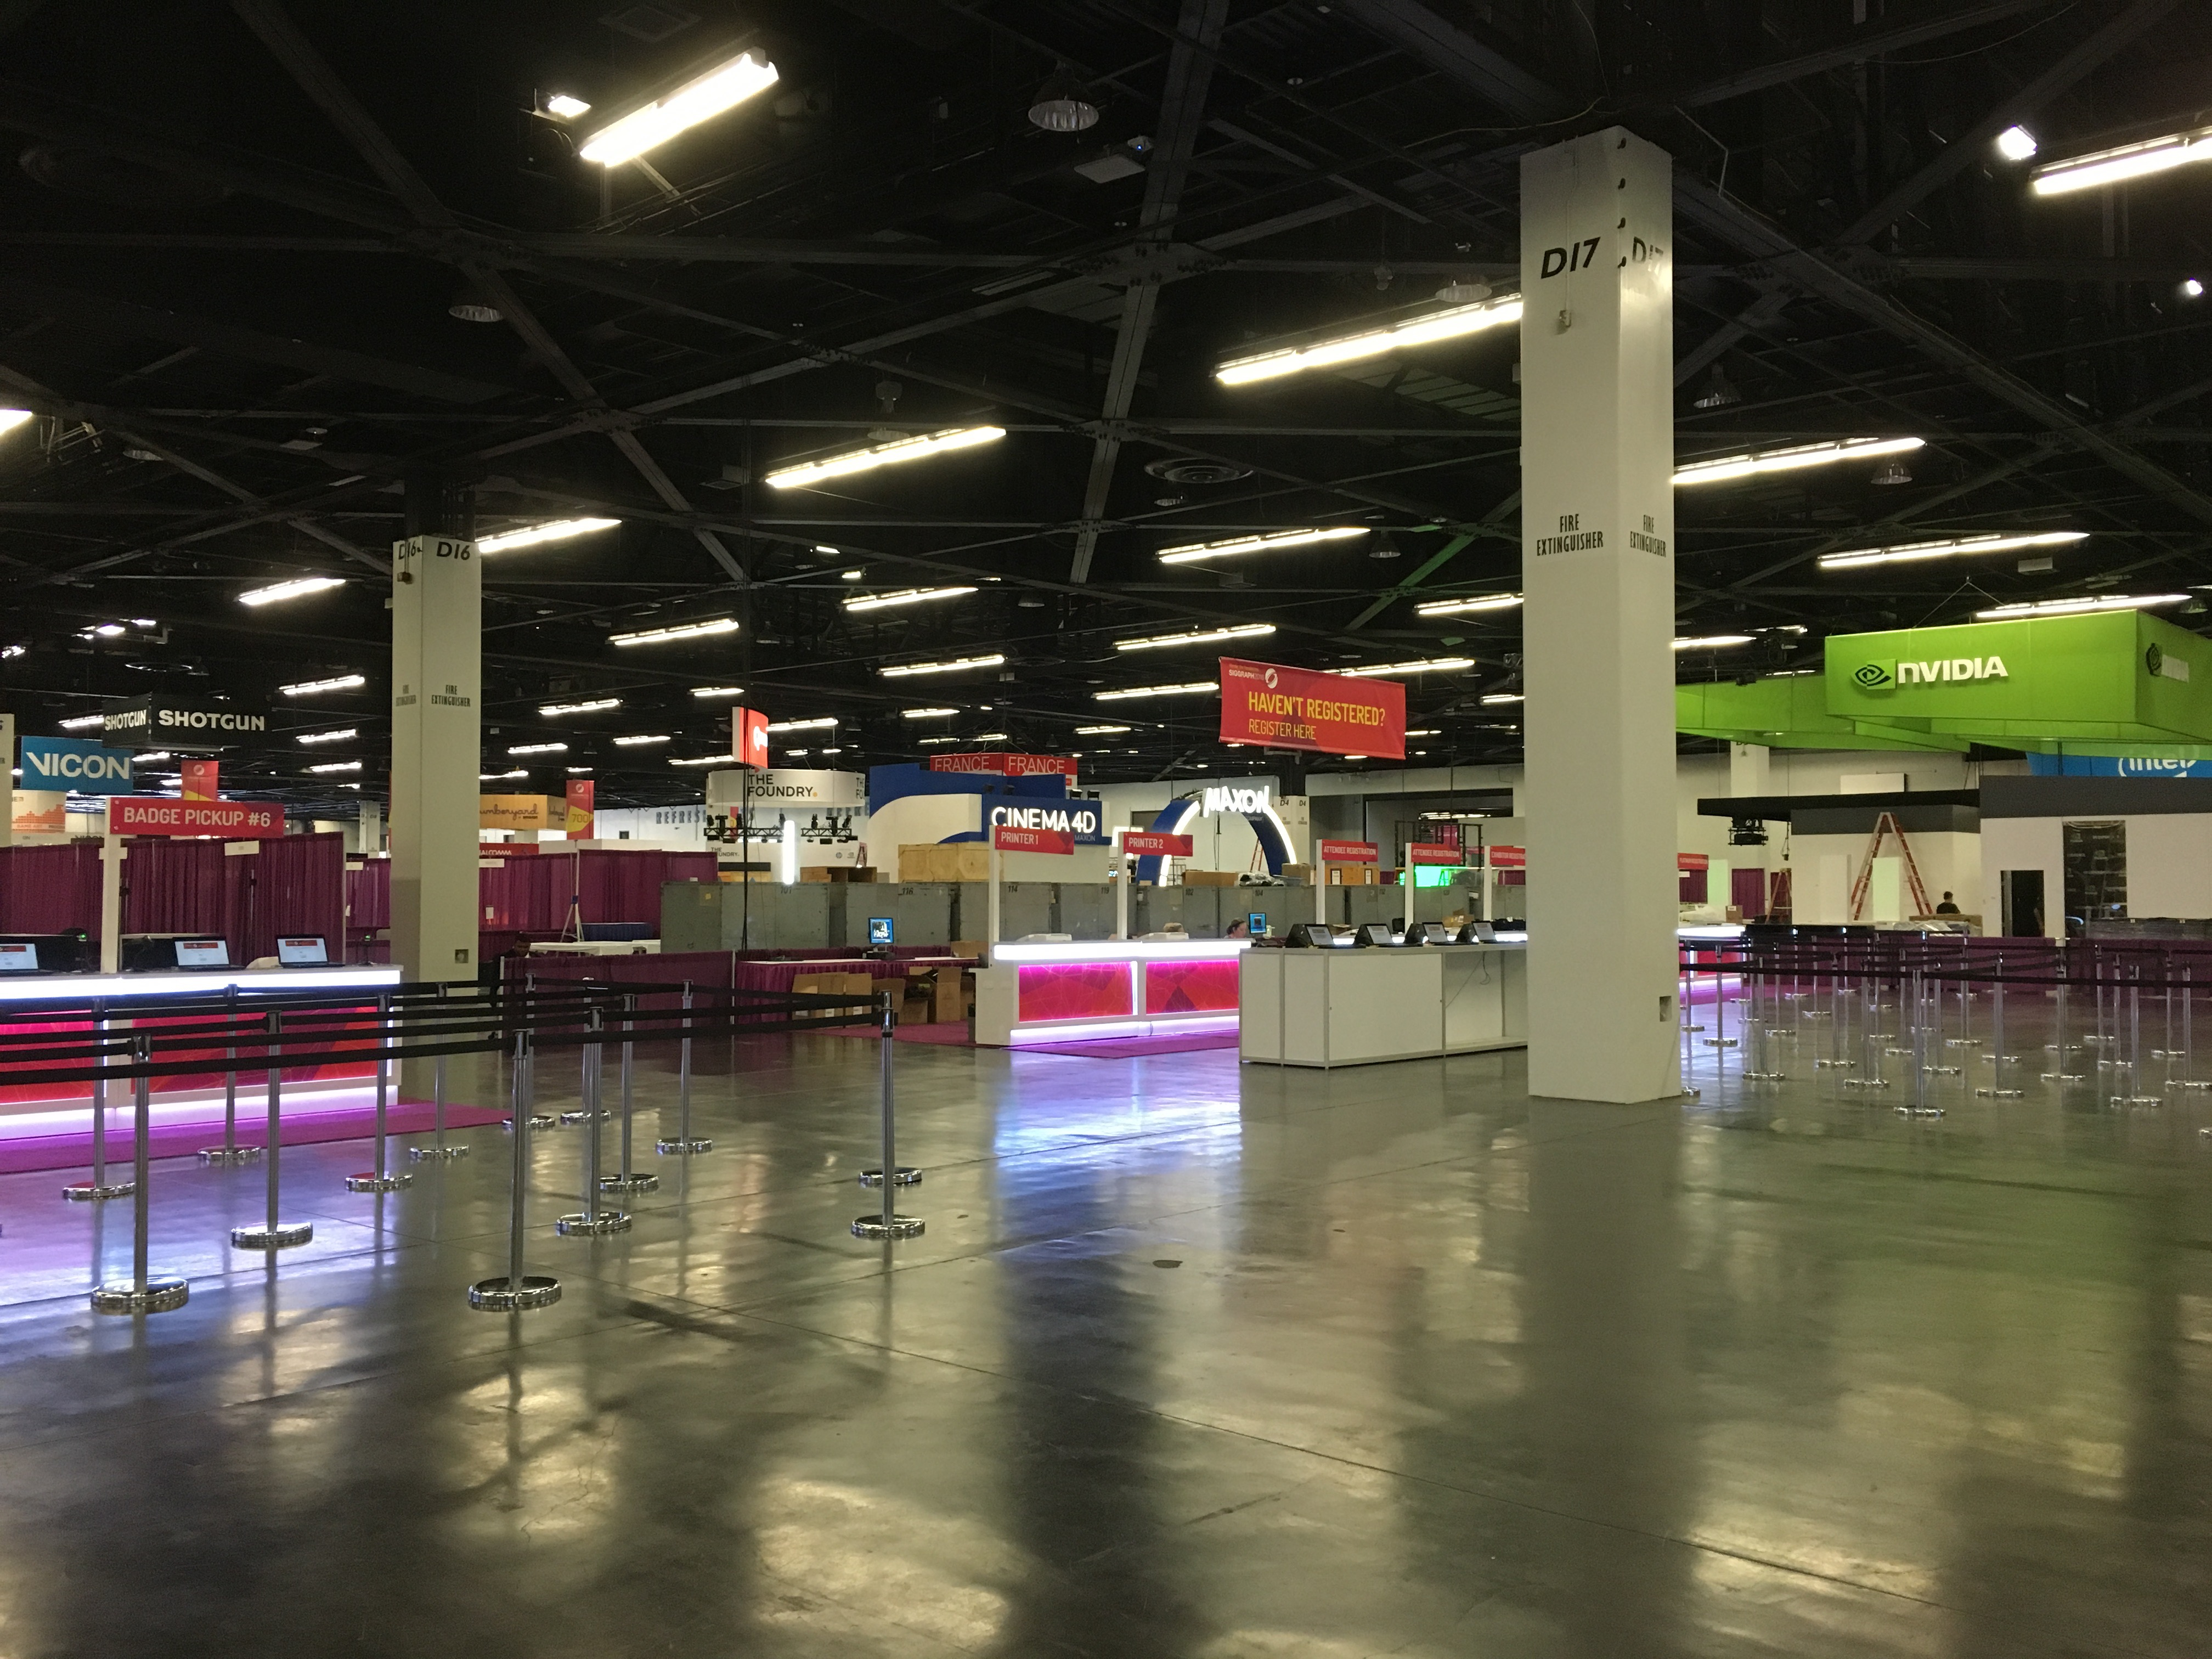
\includegraphics[width=\textwidth]{saturday_setup}
	\caption*{Exhibition Hall.}
\end{figure}

You are more than happy to keep your hands busy, as this will be a day of sitting and waiting interspersed with standing and waiting. You chat with other students as you fall into the rhythm of collecting papers in order and stuffing them into a tote before flopping it on a \textit{done} pile. Some of other SVs you chat with are still in school studying animation or computer science; one is established at MPC, working on pipeline tools related to rendering. It is at this point you sense the tension that naturally exists between the students rearing to go into industry and the folks who are fortunate enough to already have jobs. The overwhelming majority of folks you meet are students either headed towards the job hunt or beginning to grow frustrated by the post graduation struggle. You consider yourself among the fortunate, hoping to never come across as standoffish as the one girl who's job was admittedly about as good as one could hope for in this industry as a student fresh out of college. You swap contact info and ask her to send you some book recommendations related to rendering, since she mentioned she is rapidly trying learn the necessary fundamentals for her work along the way. Her business card is fancy, but not nearly as creative as the ones you will receive from budding artists you meet throughout the week. You feel dumb for not printing business cards even though you are not looking for a job. Small oversight. As noon approaches, you excuse yourself to head upstairs for check-in and registration. You didn't arrive several hours early just to be late.

During check-in you fall in with a group that develops out of the people who happen to be standing in line near you---a line containing a few hundred student volunteers that will take nearly 2 hours to deliver you to a table where you are handed a conference badge, two orange DreamWorks Student Volunteer shirts, and a whiteboard on which you write your name before having your mugshot taken. As you snake in from a lobby along the long wall of the hall where badges and other items are distributed, showreels on smart phones and clever business cards come out. You are impressed by this work, especially the 2D drawings that every artist seems to have in their scrollable portfolios. What you see is breathtakingly imaginative---a whole other world from what you are used to. Frankly, you're a bit envious, because to sit and dream and render on the page what comes into your mind seems a skill that you desperately need in your life. In fact, it is not the skill you wish you could develop---you just wish you could communicate the things you see alongside words. You wish you could express yourself in this way, let alone draw something interesting. What you see isn't just an example of tecnical skill. You see raw creativity in these shared portfolios and it is exciting to see someone's personality and hard work right in your own hands as you cradle their phone, swiping, pausing, and swiping again. You make a point to tell anyone whose portoflio you see what exactly stood out to you and why. In terms of visual output, the only thing you would be proud to share is your street photography, via Flickr. And you have shared this with friends, and it is a vulnerable thing to share your work. You know how much it means to you when someone actually engages your work, rather than acknowledging that you \textit{made a thing}. If there's one thing you can say, it is that despite your humble artistic abilities, you do know how to engage someone's work and explain what you think. You are hungry for experiences like this, and the time in the line passes quickly.

You hear a lot of discussion on the topic of 3D modeling and recognize the bandwagon everyone seems to be clamoring to hop onto. You sense a lot of this effort is misguided. One girl has taken up an interest in motion graphics in the sports entertainment industry---EA is a company she is gunning for. Another girl is interested in Naughty Dog, their art style apparently something she feels she is a good match for. Another guy has been spending his time modeling hospital tools and you think he doesn't really have much direction to his work; he is now desperately tyring to flesh out a portfolio in the hopes of finding a job. You are not an artist and cannot help but be humbled by both the incredible talent and the daunting challenge of actually entering the industry your fellow student volunteers aspire to join. Again, you feel fortunate for your line of work. You continue to take pride in introducing yourself as a software engineer now living happily in Boulder, beginning to get acquainted with the CAD industry and spending your free time reading and riding your bike in the mountains. You're a recent grad for whom your academic track is at least proven somewhat: you have a job and your job is an interesting one where you can continue to learn. That counts for a lot. You are grateful for your current station. You understand that this isn't always comfortable for those still searching to hear. Like you several months before SIGGRAPH, they may be wondering how in the hell they will take what they feel to be a decent amount of experience and parlay that into a real job doing something related to what they love or happen to be skilled at. They feel like they can do great work, and yet they are still searching. The angst is as palpable as the BO that will creep up on you in the crowds at SIGGRAPH throughout the week.

Perhaps some write you off as just a technical guy, on account of the engineer buzzword popping up. You don't hear others introducing themselves as an engineer. Ok, that one girl who works at MPC and a guy you will befriend who knows a thing or two about game engines. But other than that, everyone here does art---some tout the latest and greatest in tooling and others cling to their notebooks, but their work is \textit{art}. You don't really have anything flashy to show, save a neat animation or two from your projects developed during Chris Tralie's course. You are proud of what you have done recently, but you see the slight culture mismatch and understand that not everyone will be impressed by what you do. It is nice to hear many are familiar with the product you help to develop. A lot of the shop names people will toss out are unknown, or at least not household names. One girl from your school is working at DreamWorks, but that is not the norm. You grow bored of conversations centered on the current suite of tools each student is trying to learn and efforts to expand portfolios in the months following graduation. Eventually you get your badge and stop fretting over whether you will be swimming in your medium-sized SV shirts. Your uniform: tucked in orange DreamWorks shirt identifying you as a SV, neon green Nvidia Lanyard, messenger bag, Field Notes in the back pocket, and a mechanical poking out of your pocket.

Between check-in and orientation in the late afternoon, you are free to kill some time. You join several of the people you were talking to in line and grab mediterranean food near Harbor Boulevard and Katella. Out of this particular group, you get along well with a woman who is 12 years her sister's senior. She is a special education teacher in Oklahoma. You bend her ear with your thoughts on education and the two of you get along well. After hearing your own story describing your motivations and acculturation throughout high school, she seems quite fond of you and tells you she is going to use your story. You appreciate talking with people like her. She is decidedly the adult among the other students and although she is only visiting throughout the week while her younger sister serves as a SV, you feel a draw towards hanging out with people like her instead of the overly eager students you have encountered so far. You know why this is: you aren't here to get a job. You are here to see some cool shit and learn about things that you didn't know existed before. You want to sit down and talk with adults, not play Pokémon Go during downtime with the other SVs. You feel you have matured over the last few months and understand that a relatively small group of the Student Volunteers are at a similar stage of life as you. Many of the students are on a timeline one year behind you. That's okay, but in that one year a lot changes. Fortunately, you find a group later on in the week that you feel comfortable with and in which you feel you can talk about the things you currently care about.

Orientation itself is a matter of sitting in a large hall and listening to various officials introduce one another for a little over an hour. This isn't painful, because Christian Wittorf, the Student Volunteer Program Chair, happens to be a tremendously funny speaker. You review various protocols describing how to interact with attendees and where to find critical information or how to swap volunteer shifts through a large powerpoint and call-out-the-answer responses. After a Q\&A session, you are all shuffled out to the main fountain in front of the Convention Center where a picture is taken. As you are assembling on the fountain you run into a girl who just graduated with you from your school and happened to be in two of your classes during your last semester. She just started working at DreamWorks out in Los Angeles. During the commotion you meet several other students. After the picture, there is pizza, and you feel awful after a few slices, but you couldn't resist.

\begin{figure}[h]
	\centering
	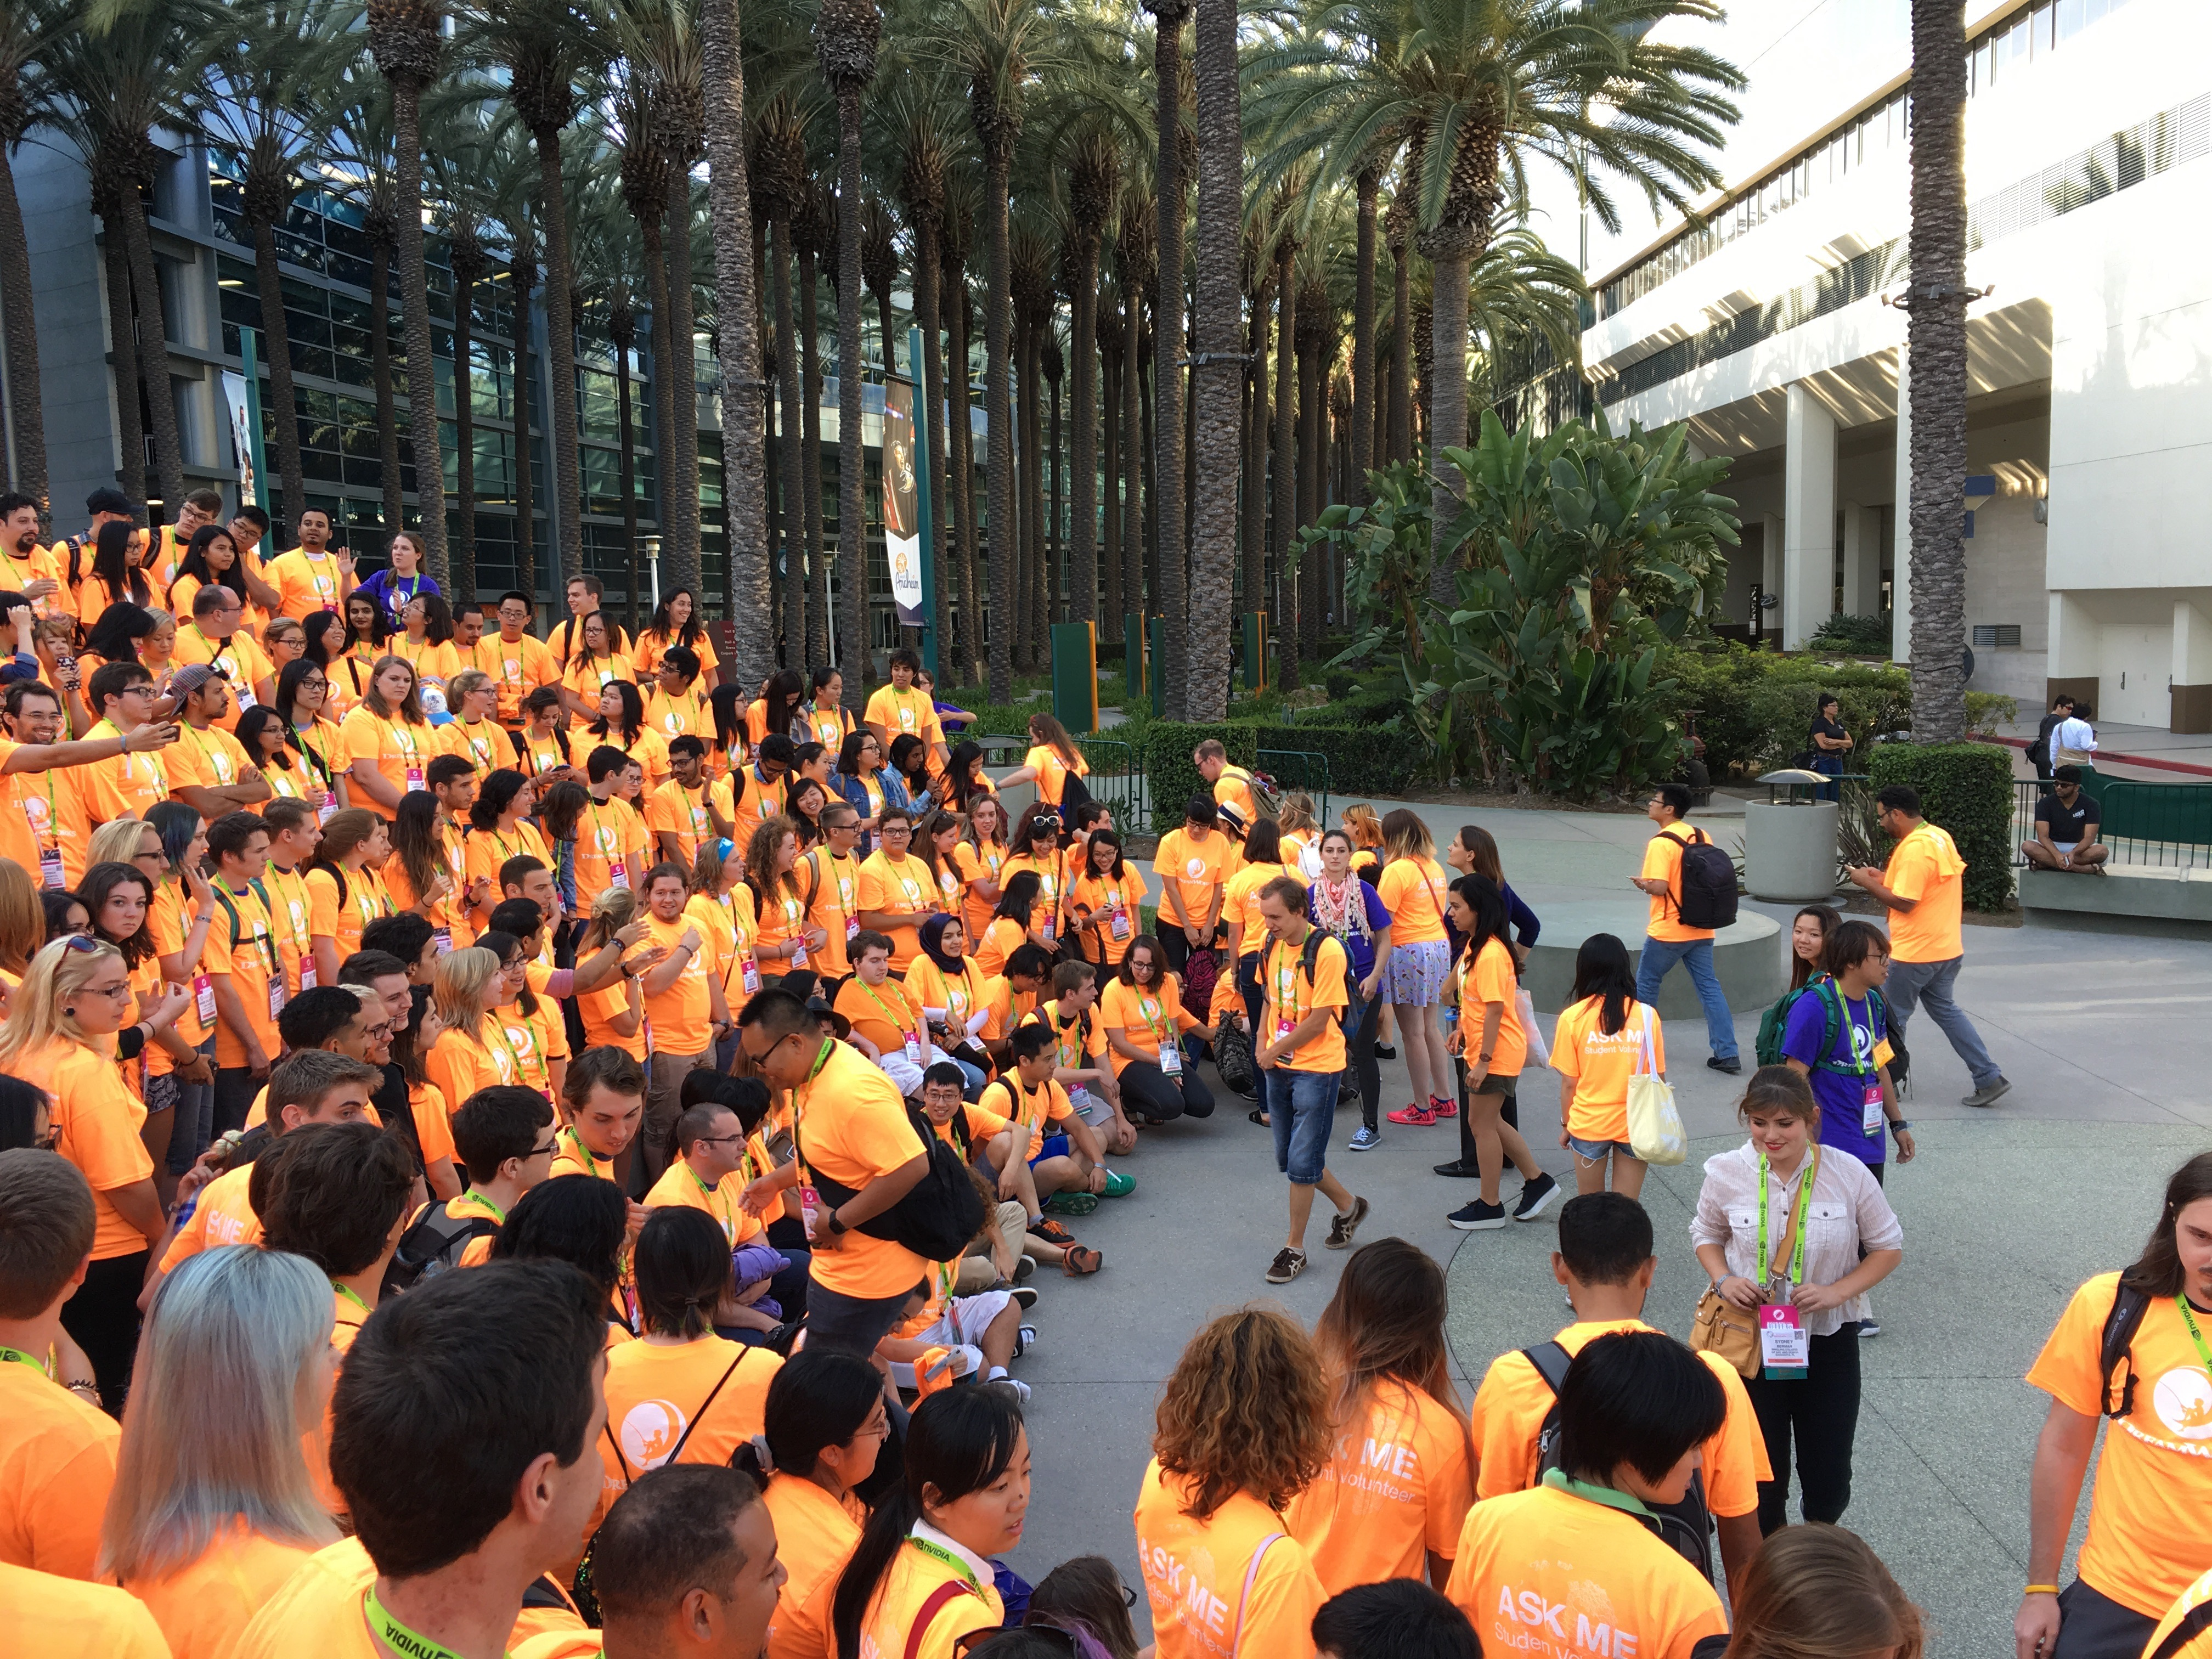
\includegraphics[width=\textwidth]{picture}
	\caption*{Group picture in front of the Anaheim Convention Center.}
\end{figure}

As is the nature of big events, pacing yourself can be difficult, and several students organize a party to follow the pizza somewhere in Downtown Disney. You learned of this from the Facebook group: an event had been maded and the number attending seemed promising. You don't want to be left out, so you end up walking a mile with a group of other attendees to a place where you expect to eat and possibly grab a drink. Along the way, you continue a conversation with a girl you met earlier. You both talk about favorite books and your writing experiences. She studied English in Oregon and is in a masters program at the The University of Edinburgh, where she has developed several video games that you will end up playing upon your return and completing surveys for. You both seem to respect each other's love for tech and the humanities. You talk for a while about her storytelling efforts in her games which, again, you swear you will play and in fact not only play through, but complete surveys for when SIGGRAPH is over. This young lady is incredibly impressive, writing the scripts for her games as well as programming them in Unity. You are maybe just a little bit smitten by the end of the walk from the Conventon Center to the meetup that has been advertised on the Facebook group.

\begin{figure}[h]
	\centering
	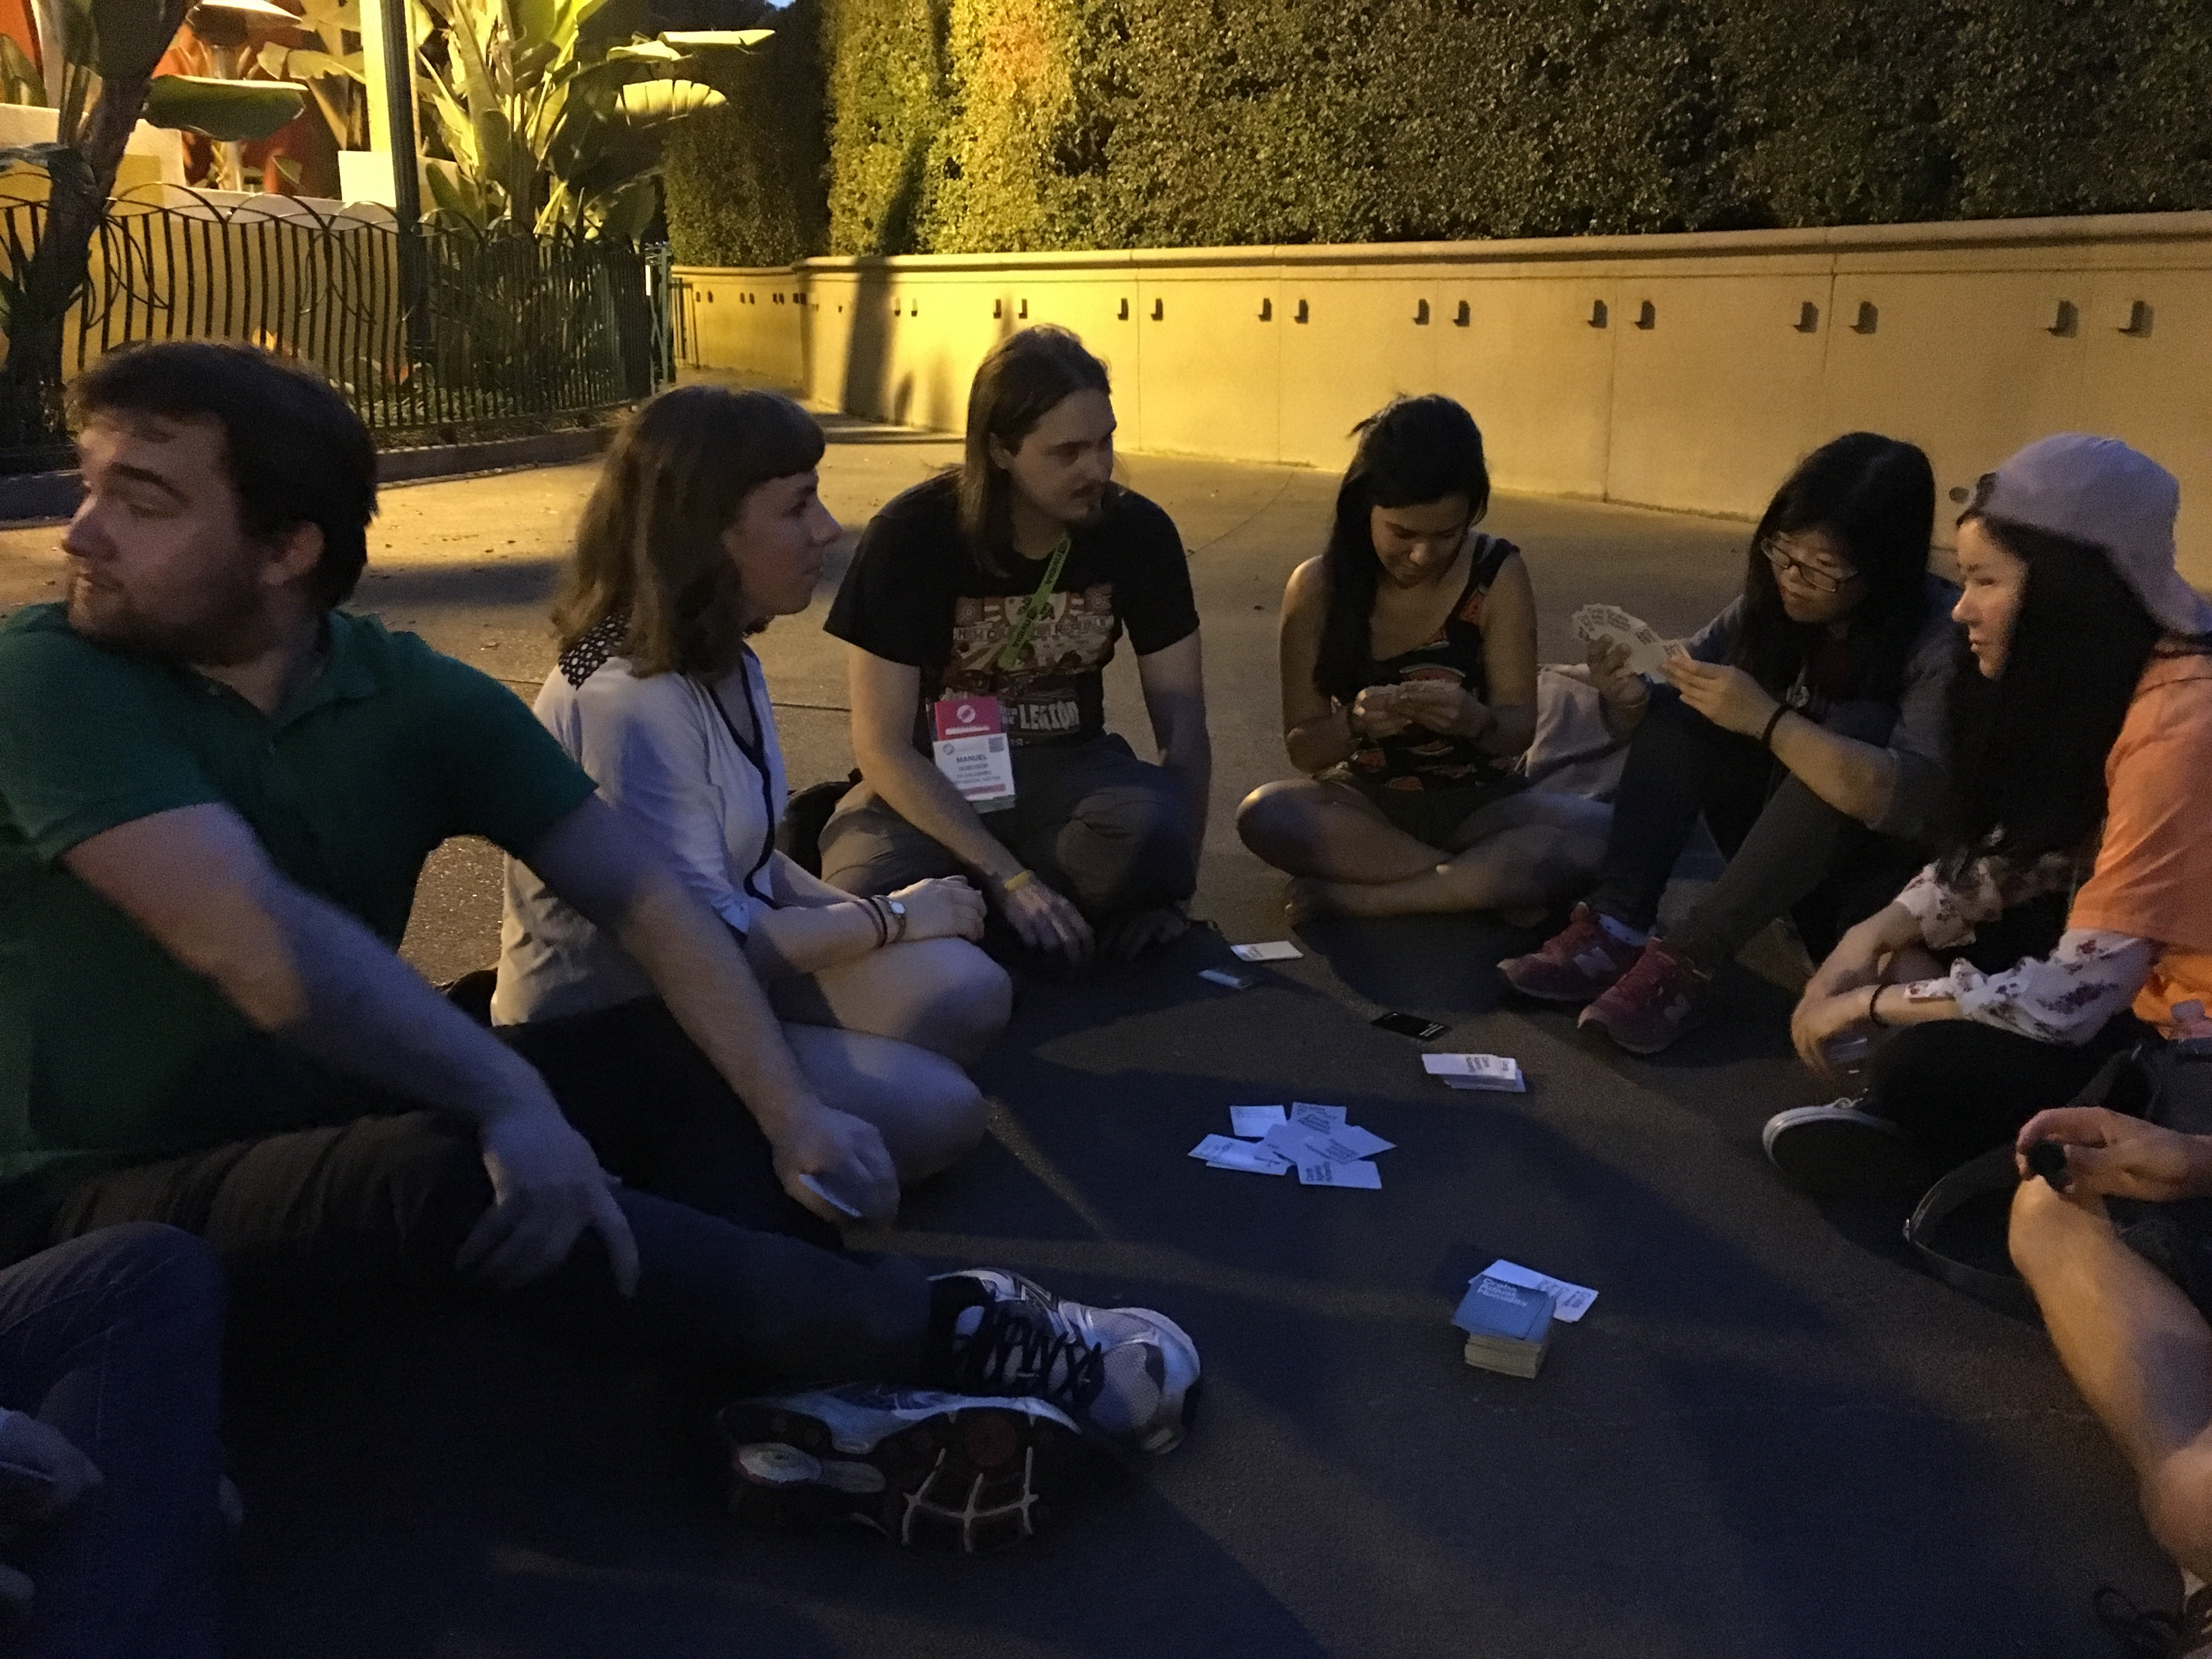
\includegraphics[width=\textwidth]{cards_against_humanity}
	\caption*{Cards Against Humanity in the middle of Downtown Disney.}
\end{figure}

Arriving in Downtown Disney, you are disappointed to find the wait time is nearly forever and the only actual activity the person who had created the Facebook event has planned is to hand out many decks of \textit{Cards Against Humanity} (and \textit{Crabs Adjust Humidity}) so that groups of a dozen or so SVs can sit down on the pavement outside a restaurant off the main throughfare of the park. To play cards. You had hoped to actually have a drink and continue picking your new friend's brain. The game quickly wears on you, with English as a second language students more or less butchering any fun to be had in Cards Against Humanity's references. And you \textit{love} Cards Against Humanity. You end up leaving with a group of students who will eventually become your main crew for the rest of the week in search of a dive bar to post up in. It's time to socialize and make friends, and that was not happening during the card game. Or at least the friends you were hoping to meet were the sort of friends who would get up in search of something else to do in Downtown Disney, as these SVs had done. So you tag along. For some reason you feel tonight is the night to create some bonds for the rest of the week. Failing to find a bar after being led astray by an assumed leader of the pack, you are all treated to fine display of the daily Disney fireworks from the parking lot of an Anaheim restaurant.

You all decide to try again another day and you have an Uber take you back to your host's house a short 15 minutes away. You hadn't really been after a drink, but rather a place less \textit{Disney} than where your journey had taken you. You love to talk with people to really get to know them, and you hope the rest of the week will let you get closer to some of the people in your group who were similarly disapointed. A lot of the SVs remind you of your experiences with the People to People program. You have changed a lot since you went abroad back in middle school, but today has brought you back to those weeks spent among similarly aged students with matching shirts and lanyards bumbling as an awkward herd through new sights and places. You fall asleep like a candle had been snuffed out.

\end{document}